\chapter{Design}
	
	After the security audit, it was apparent that the majority of the codebase needed to be refactored in order to make it object-oriented.
	The decision to rewrite the program was not a light one, by rewriting the program, the scope of extensions to \ac{AWESOME} became much more limited via time constraints.
	
	With the rewrite came the opportunity to utilise both a framework and a design pattern.
	Frameworks were ruled out under the stance that it had to be deployed on a server without shell access.
	However later research discovered that this is achievable in Laravel\footnote{Laravel Homepage: \url{http://laravel.com}}, which would have been the framework of choice for several reasons.
	
	Laravel would have provided a complete, and mature \ac{MVC} framework, as well as an \ac{i18n} framework and a solid basis for \ac{AWESOME}.
	Ultimately, poor research into Laravel on a shell-less server resulted in an attempt to produce a bespoke \ac{MVC} framework, which, unsurprisingly is harder than it first seems.
	
	\section{Programming Language}
	
	The programming language choice was fairly fixed, as it had to be easily runnable on an \ac{AU} server.
	This limited the choice to PHP, but which minor version of PHP was only found out later in the project which is discussed further in \autoref{sec:auserverimp}.
	
	If this requirement wasn't an issue, using Ruby with the Rails framework would have been a great candidate for this project, as rails already provides a mature \ac{MVC} framework, many third-party gems for \ac{i18n}, and many other language-inherent features, such as better type safety, and integrated testing tools.
	
	Ruby on Rails can also perform background tasks, unlike PHP, which can be really useful when handing large volumes of mail, such as those sent out to students with unique questionnaire links.
	
	\newpage
	
	\section{\acl{MVC} Framework}
	
	Since using a ready-made framework was ruled out, a custom-made \ac{MVC} framework was written to support this project.
	The design of which is laid out in this section and is very heavily taken from the `Write your own PHP MVC Framework' series of tutorials\cite{php-mvc-tutorial}.
	
	\subsection{Routing}
	
	URL Routing is a way to access specific controllers and views from a URL.
	This works via an Apache rewrite rule, which appends a \$\_GET variable which contains the current requested URL.
	
	The URL routing is handled as such: \textit{awesome.url/controller/view[/query]}
	
	By using routing in the URLs, we can eliminate the `messy' looking get parameters in the URL, and have nice clean looking links.
	
	\subsection{Directory Structure}
	
	\autoref{fig:mvcdirtree} shows the directory structure of the \ac{MVC} framework.
	
	`\textit{src}' is the source code to the program. Inside it contains everything needed to run \ac{AWESOME}.
	
	Inside `\textit{tests}' are the unit tests to be run automatically by TravisCI and PHPUnit.
	
	`\textit{src/app}' has the MVC classes (controller, models and views) which are used when the routing engine rewrites URLs.
	
	`\textit{src/config}' contains the config file for the program.
	In this file, database credentials are set, as well as SMTP mail server settings, some \ac{i18n} settings, and the debug flag which displays errors and shows a feedback form/notice (See \autoref{fig:feedbackform}).
	
	`\textit{src/db}' is a directory for \ac{SQL} dumps for the database schema.
	
	`\textit{src/i18n}' contains translation files for the \ac{i18n} framework, but more detail is in \autoref{sec:i18nframework}
	
	`\textit{src/lib}' is the `glue' that holds the MVC framework together.
	It contains the autoloader class, the bootstrap script, a \ac{PDO} database class, and the third-party, open source PHPMailer\cite{phpmailer} classes used for sending mail via SMTP.
	
	`\textit{src/logs}' is where any PHP errors get logged when debug mode is off. This is in order to hide any potential security issues with displaying errors.
	
	`\textit{src/public}' is the main entry point to the program and where the Apache vhost will be set.
	
	`\textit{src/public/assets}' contains the Javascript, SASS, CSS, and images used in the HTML.
	Users visiting the public directory with a valid token will be taken to their corresponding questionnaire.
	
	`\textit{src/public/admin}' is protected by HTTP authentication to prevent anybody from creating surveys and sending them out, or reading the results of previous surveys.
	
	\begin{figure}[H]
		\dirtree{%
			.1 AWESOME.
			.2 src.
			.3 app.
			.4 controllers.
			.4 models.
			.4 views.
			.3 config.
			.3 db.
			.3 i18n.
			.3 lib.
			.3 logs.
			.3 public.
			.4 admin.
			.4 assets.
			.2 tests.
		}
		\caption{Directory structure of the \acs{MVC} Framework}
		\label{fig:mvcdirtree}
	\end{figure}
	
	\section{Internationalisation Framework}
	\label{sec:i18nframework}
	
	The \ac{i18n} framework is a tiny standalone \ac{OOP} module which utilises JSON formatted files with strings for translation.
	JSON was chosen as it is easily human-readable, is easy to manually create, and not verbose enough to put off a non-programmer from modifying it.
	This means that even people not familiar with JSON can still easily provide translation files for \ac{AWESOME}.
	
	The JSON files are structured like the one in \autoref{fig:i18njson}. The first two entries are \ac{i18n} metadata, for ISO639-1 code\footnote{ISO639-1: \url{http://en.wikipedia.org/wiki/ISO_639-1}}, and language.
	Each string has an ID, and a translation string to be returned.
	Every language uses the same ID, and what gets returned depends on the language set via a global variable.
	
	The \ac{i18n} class has a global function, \_\_(\$string\_id) which will then return the appropriate translated string depending on the \$lang global variable.
	
	\begin{figure}[H]
		\begin{verbatim}
{
    "@ISO639-1" : "en",
    "@lang" : "English",
    "invalid-url" : "The URL provided is incorrect.",
    "send-responses" : "Send Responses"
}
		\end{verbatim}
		\caption{JSON Format for \ac{i18n} language files.}
		\label{fig:i18njson}
	\end{figure}
	
	\section{Database Schema}
	
	The database schema (see \autoref{fig:schema}) used is very similar to the prototype version.
	Documentation needed to be written for the existing schema, so the opportunity was taken to make some changes in the structure of the database before this happened.
	The old database schema did not use any foreign key constraints, nor was the use of primary keys ideal.
	
	Foreign keys are very useful to have in a system like this, as orphaned rows can be cleaned up nicely with a cascade delete.
	This prevents any data remaining in the table incase it is missed by an \ac{SQL} query that hasn't been updated in the code.
	
	Some changes were made to the way things were named, mostly to prevent confusion.
	In the new schema, a survey is a set of questionnaires, each of which is tailored to a specific student.
	In the old schema, everything was called a questionnaire, which led to confusion between a group of questionnaires and a single questionnaire.

	Additional changes need to be made in order for \ac{AWESOME} to support multiple departments across the university, but this is out of the scope of the dissertation, although this feature is on the roadmap if \ac{AWESOME} is to be used university-wide.
	
	\begin{figure}[H]
		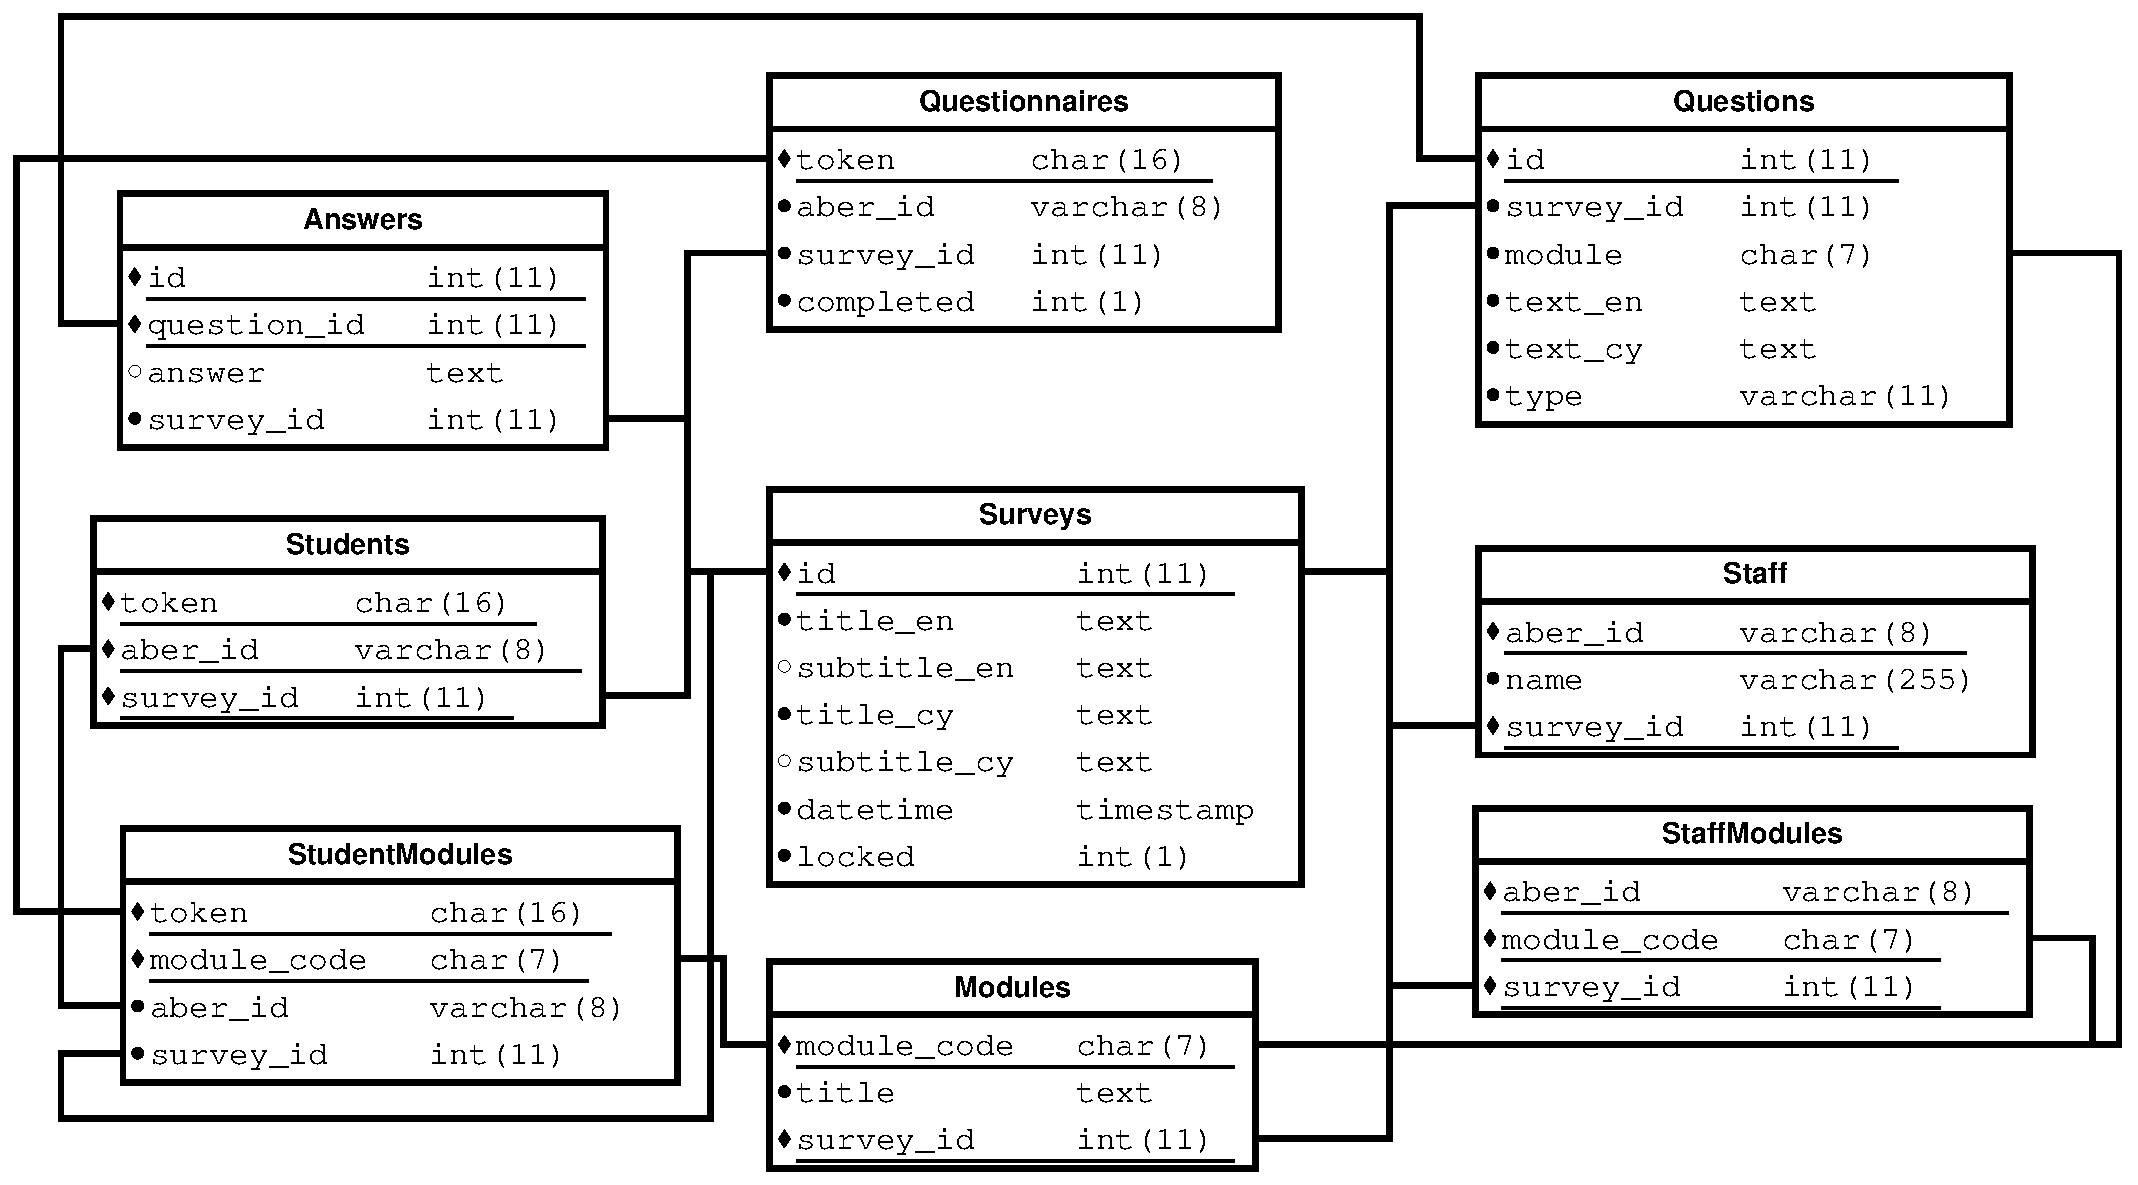
\includegraphics[width=\textwidth]{schema}
		\caption{\ac{AWESOME} database schema design.}
		\label{fig:schema}
	\end{figure}
	
	\section{User Interface}
	
	The user interface was fairly polished on the respondent-facing sections in the prototype, so a lot of elements were re-used in that, with a few minor changes to visual aspects to improve readability, as can be seen in \autoref{fig:questionnaire-comparison}.
	
	The admin dashboard of the prototype wasn't very user friendly, creation of a survey was split over several pages which didn't need to be separated.
	This resulted in the creating of surveys, adding questions, modules, students, and staff being quite convoluted and not straight-forward.
	Results weren't clear to look at either, and took up a lot of space per-question by pie charts, which were unnecessary given the type of data provided.
	
	\autoref{fig:surveys-comparison} shows the main dashboard screen, which contains a list of all surveys.
	In this list, the survey name, description, response rate, date and locked status are displayed.
	By displaying the response rates in here, you can easily see progress of the surveys, and quickly gauge the response rate of students for a particular survey.
	
	\autoref{fig:results-comparison} shows the difference in results pages.
	Information density is a lot greater in the new version and it makes it much easier to see the results of Likert scale questions at a glance.
	Textual comments have a large presence for good reason in the results page, as often they provide the most valuable information about a module.
	If comments were hidden behind a scrollable frame, comments may be overlooked or missed.
	
	\begin{figure}[H]
		\includegraphics[width=\textwidth]{screens/prototype-questionnaire}
		\includegraphics[width=\textwidth]{screens/final-questionnaire}
		\caption{A comparison of questionnaire pages between the prototype version and the submitted version of \acs{AWESOME}}
		\label{fig:questionnaire-comparison}
	\end{figure}
	
	\begin{figure}[H]
		\includegraphics[width=\textwidth]{screens/prototype-viewall}
		\includegraphics[width=\textwidth]{screens/final-viewall}
		\caption{A comparison of surveys view between the prototype version and the submitted version of \acs{AWESOME}}
		\label{fig:surveys-comparison}
	\end{figure}
	
	\begin{figure}[H]
		\includegraphics[width=\textwidth]{screens/prototype-results}
		\includegraphics[width=\textwidth]{screens/final-results}
		\caption{A comparison of results between the prototype version and the submitted version of \acs{AWESOME}}
		\label{fig:results-comparison}
	\end{figure}
	
	\begin{figure}[H]
		\includegraphics[width=\textwidth]{screens/prototype-single}
		\includegraphics[width=\textwidth]{screens/final-questions}
		\caption{A comparison of survey view between the prototype version and the submitted version of \acs{AWESOME}}
		\label{fig:view-comparison}
	\end{figure}
	
	\begin{figure}[H]
		\includegraphics[width=\textwidth]{screens/prototype-respondents}
		\includegraphics[width=\textwidth]{screens/final-respondents}
		\caption{A comparison of respondents between the prototype version and the submitted version of \acs{AWESOME}}
		\label{fig:respondents-comparison}
	\end{figure}
		
	\autoref{fig:view-comparison} shows the great difference between the two survey page designs.
	The newer one has all of the information contained in four tabs in the page, as well as being able to easily see response rate again.
	Questions are in collapsible panes to easily separate the three different types of questions available and provide additional information if required.
	
	\autoref{fig:respondents-comparison} shows the Respondents tab in the new version, compared to the old respondents page.
	As you can see, the colour coding of completed/incomplete makes a large difference in the availability of data at a quick glance, and also matches the response rate bar's colour scheme.
	This is the page that can be used to chase up students who fail to answer the survey as well as reward students for completing it.
	Targeted reminder emails can be sent from here to only those who have not yet completed their questionnaire.
	
	\begin{figure}[H]
		\includegraphics[width=\textwidth]{screens/prototype-csv}
		\includegraphics[width=\textwidth]{screens/final-csv}
		\caption{A comparison of CSV input between the prototype version and the submitted version of \acs{AWESOME}}
		\label{fig:csv-comparison}
	\end{figure}
	
	\autoref{fig:csv-comparison} shows the drastic difference between the prototype CSV import and the new one.
	The prototype version has one page per CSV file.
	This is a slow process to go through to get data imported, what would be much nicer is if you could copy and paste directly into fields on the same page and submit them all at once.
	This is what the submitted version does, and it does it quite well too.
	It's very fast at getting data into the system.
	
	Additional features include a feedback form (\autoref{fig:feedbackform}) when \ac{AWESOME} is in debug mode.
	This allows users to send an email to developers, containing any text they wish, as well as automatically including user-agent and other metadata to help identify the problem.
	
	\begin{figure}[H]
		\centering \includegraphics[width=0.33\textwidth]{screens/i18n-selector}
		\caption{A screenshot of the \ac{i18n} selector in \acs{AWESOME}}
		\label{fig:i18nselector}
	\end{figure}
	
	\begin{figure}[H]
		\includegraphics[width=\textwidth]{screens/final-feedbackform}
		\caption{A screenshot of the feedback form in \acs{AWESOME}}
		\label{fig:feedbackform}
	\end{figure}
	
	\begin{figure}[H]
		\includegraphics[width=\textwidth]{screens/final-about}
		\caption{A screenshot of the about dialog in \acs{AWESOME}}
		\label{fig:aboutpage}
	\end{figure}